\section{Hybrid Programming using MPI+MPI$_{sm}$}
The idea of hybrid programming consist of combining parallelization between nodes with parallelization inside SMP nodes. Traditionally, parallelization between nodes is being achieved using distributed memory programming model such as MPI, while parallelization inside SMP nodes is achieved using shared memory programming model such as OpenMP, posix threads, or MPI$_{sm}$. In this section we will present preliminary results that allows to compare a couple of hybrid implementation of the Jacobi iteration program introduced in the previous section. The comparison also includes results obtained from a traditional (non-hybrid) MPI version of the same program.

\medskip

\subsection*{Hybrid programming in MPI}
While in the hybrid programming combining MPI and OpenMP (MPI+OpenMP), it is usual to have several OpenMP threads inside a node and (frequently) one MPI processes per node, in the MPI+MPI$_{sm}$ hybrid programming everything is an MPI process. Therefore, the MPI+MPI$_{sm}$ hybrid programming requires a mechanism to distinguish between processes that exist inside a node and those belonging to different node. Therefore, this section start with a brief description of MPI function and datatypes that can be used to accomplish this goal. The pseudo code bellow can help to describe the important steps in this process. 

\medskip
Two variables of type MPI\_Group, one for the whole set of ranks and one for the ranks belonging to a node are needed. This is shown in line 7 of the pseudo code. These variables are used to define global and shared group communicators using the MPI\_Comm\_group() function as shown in lines 8 an 9. 


\begin{lstlisting}[style=CStyle]
#include <stdlib.h>
#include <stdio.h>

int main(int argc, char *argv[]) 
{
    .
    MPI_Group sharedGroup,worldGroup;
    MPI_Comm_group(MPI_COMM_WORLD, &worldGroup);
    MPI_Comm_group(sm_comm, &sharedGroup);
    .
    int *partners, *map;
    partners = (int *)malloc( worldSize * sizeof(int) );
    map      = (int *)malloc( worldSize * sizeof(int) );
    .
    MPI_Group_translate_ranks(worldGroup, worldSize, partners, sharedGroup, map);
    .
    if (map[myWorldRank+1] != MPI_UNDEFINED) {
        memcpy(&Temperature[(nRows)*COL2],&Temperature[(nRows-2)*COL2],...);
    } else {
        MPI_Irecv(&Temperature[(nRows-1)*COL2],....);
        MPI_Isend(&Temperature[(nRows-2)*COL2],....);
        MPI_Waitall(2,request, status);
    } // end if //  
    return 0;
} // end main() // 
\end{lstlisting}


Also needed are a couple of integer pointers which need to be allocated to the size of the MPI\_WORLD\_COMM (the total number of MPI processes used for the program), lines 11 to 13. These pointers are used to map global rank numbers to shared rank numbers using the function MPI\_Group\_translate\_ranks(), shown in line 15. The \emph{map} pointer is of special interest. Each element of this pointer represent each one of the MPI processes used by the program. After the MPI\_Group\_translate\_ranks() is called, all the elements of the \emph{map} pointer, except those corresponding to processors belonging to a given node are set to an undefined state (MPI\_UNDEFINED). This can be used to determine the type of communication a given process can have with another process depending on the location (inter-node vs intra-node) of that process, as shown in lines 17 to 23.


\subsection*{Jacobi iteration - MPI and Hybrid Results}



Figure \ref{fig:Figure5} shows results comparing the performance (time) of two hybrid implementations as well as the traditional MPI case running in 16 Blue Waters Nodes. 



The programs are solving a 4096 X 4096 grid. The hybrid versions of the program sub-divide the grid, by rows, in 16 parts, handling each of this parts in a separate node. Therefore they have only communication among the nodes (inter-node communication). Inside each node the hybrid versions use an increasing number of threads (OpenMP) or processes (MPI$_{sm}$) to handle their part of the problem without any communication involved.

On the other hand, the MPI version brake the gird in as many parts as total MPI rank are used in the solution; for example for the 256 total ranks, there are 256 MPI communication boundaries to deal with. Although most of the communication corresponds to intra-node boundaries, those intra-node communication are handled by the send/receive family of MPI functions. Additionally, the MPI version still have to deal with 16 communications corresponds to the original 16 inter-node boundaries.


%Since the amount of communication the main difference between the "pure" MPI and the hybrid cases, I believe that is the reason for the large drop of performance the MPI version is suffering.



%two computer programs are used to evaluate the performance of the MPI$_{sm}$ by comparing it to equivalent versions of the programs developed using OpenMP. The objective is to test the capabilities of MPI$_{sm}$ as a shared memory programming model and to evaluate its viability as an alternative to OpenMP.



\begin{comment}


\begin{outline}
    \item {\bf MPI+MPI$_{sm}$ as an alternative to MPI+OpenMP } \\
      The new share memory capabilities added to MPI permits to consider it as an alternative to other hybrid programming models such as MPI+OpenMP.
    \item {\bf Preliminary results } \\
    Examples program are developed to illustrate the use of the MPI functions for shared memory. An example consisting of a Jacobi iteration, solving the 2D-Laplace equation, a common technique to approximate the solution of elliptic PDEs within some allowable tolerance, was used to produce some preliminary results. A Hybrid program (MPI-MPI$_{sm}$) was developed and compared to versions of the program using other hybrid alternatives (MPI-OpenMP) as well to "pure" MPI versions. \\
    
    Figure \ref{fig:Figure5} shows results comparing the performance (time) of two hybrid implementations as well as the "pure" MPI case running in 16 Blue Waters Nodes. This preliminary result clearly shows the potential benefit of hybrid programming. Additionally it shows that the MPI-MPI$_{sm}$ approach can outperform the MPI-OpenMP version.
      
    \item {\bf Recommendations based in developed experience} \\
\end{outline}

\end{comment}



\begin{figure}[h!]
    \centering
    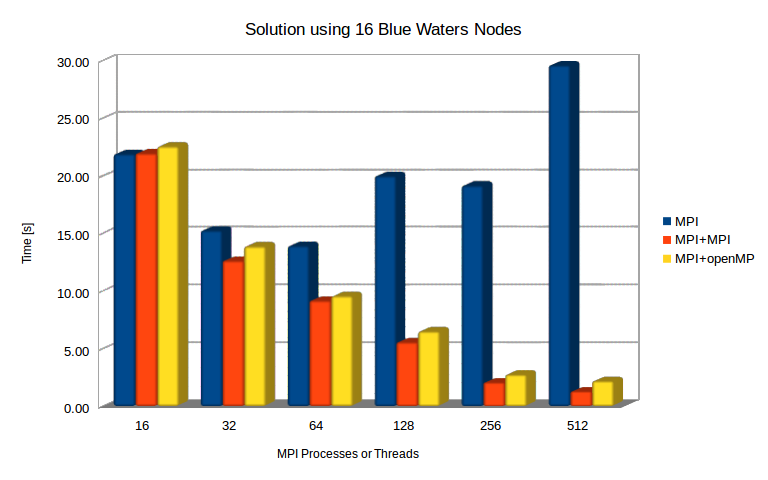
\includegraphics[width=100mm]{Plots/section4/bw2-16.png}
    \caption{Jacobi iteration solving the 2D-Laplace equation.}
    \label{fig:Figure5}
\end{figure}

This preliminary result clearly shows the potential benefit of hybrid programming, and in particular the MPI+MPI$_{sm}$ approach.

%Additionally it shows that the MPI+MPI$_{sm}$ approach can outperform the MPI+OpenMP version.
